\documentclass[preprint]{sigplanconf}

\usepackage[utf8]{inputenc}
% the following standard packages may be helpful, but are not required
\usepackage{longtable}
%\usepackage{mathtools}
%\usepackage{multicol}
%\usepackage{multirow}
\usepackage{booktabs}
%\usepackage{courier}
%\usepackage[scaled]{helvet}
%\usepackage{url}
\usepackage{listings}
%\usepackage{enumitem}
%\usepackage{mdwlist} % tighter description environment (starred)
%
\usepackage{graphicx}
\usepackage{softdev}
\usepackage{amsmath}
%\usepackage{mdwlist}
%\usepackage{pifont}
\usepackage{xspace}

\newcommand{\kalibera}{Kalibera \& Jones\xspace}
\newcommand{\krun}{Krun\xspace}
\newcommand{\hypone}{H1\xspace}
\newcommand{\hyptwo}{H2\xspace}
\newcommand{\binarytrees}{\emph{binary trees}\xspace}
\newcommand{\richards}{\emph{Richards}\xspace}
\newcommand{\spectralnorm}{\emph{spectralnorm}\xspace}
\newcommand{\nbody}{\emph{n-body}\xspace}
\newcommand{\fasta}{\emph{fasta}\xspace}
\newcommand{\fannkuch}{\emph{fannkuch redux}\xspace}
\newcommand{\bencherthree}{Linux1/i7-4709K\xspace}
\newcommand{\bencherfive}{Linux2/i7-4790\xspace}
\newcommand{\benchersix}{OpenBSD/i7-4790\xspace}
\newcommand{\bencherseven}{ARM\edd{XXX name properly if used}\xspace}

\lstset{
    basicstyle=\tt\scriptsize,
    xleftmargin=2em,
    framexleftmargin=1.5em,
    numberstyle=\scriptsize\tt\color{gray},
    captionpos=b,
    escapeinside={{<!}{!>}},
}

\SDShowCommentTags{default}  %final

\begin{document}

\title{Virtual Machine Warmup Blows Hot and Cold}

\authorinfo{Edd Barrett}
{Software Development Team, Department of Informatics, King's College London}{\texttt{http://eddbarrett.co.uk/}}

\authorinfo{Carl Friedrich Bolz}
{Software Development Team, Department of Informatics, King's College London}{\texttt{http://cfbolz.de/}}

\authorinfo{Rebecca Killick}
{Department of Mathematics and Statistics, University of Lancaster}{\texttt{http://www.lancs.ac.uk/\~{}killick/}}

\authorinfo{Vincent Knight}
{School of Mathematics, Cardiff University}{\texttt{http://vknight.org/}}

\authorinfo{Sarah Mount}
{Software Development Team, Department of Informatics, King's College London}{\texttt{http://snim2.org/}}

\authorinfo{Laurence Tratt}
{Software Development Team, Department of Informatics, King's College London}{\texttt{http://tratt.net/laurie/}}


\maketitle

\section{Introduction}
\label{sec:intro}

Many modern languages are implemented as Virtual Machines (VMs) which use a
Just-In-Time (JIT) compiler to translate `hot' parts of a program into efficient
machine code at run-time. Since it takes time to determine which parts of the
program are hot, and then compile them, programs which are JIT compiled are
said to be subject to a \emph{warmup} phase. The traditional view of
JIT compiled VMs is that program execution is slow during the warmup phase, and
fast afterwards, when \emph{peak performance} is said to have been reached
(see Figure~\ref{fig:trad} for a simplified view of this).
This traditional view underlies most benchmarking of JIT compiled VMs, which
generally aim to measure peak performance.
Typically, benchmarks are run repeatedly in a single process, then data prior
to peak performance is discarded.

The aim of this paper is to test the following hypothesis:
\begin{description}
  \item[\hypone] Small, deterministic programs exhibit traditional warmup behaviour.
\end{description}
In order to test this hypothesis, we present a carefully designed
experiment where a number of simple benchmarks are run on a variety of
VMs for a large number of \emph{in-process iterations} and repeated using fresh
\emph{process executions} (i.e.~each process execution runs multiple in-process
iterations). We deliberately treat VMs as black boxes: we simply run benchmarks
and record timing data.

\begin{figure}[t]
\centering
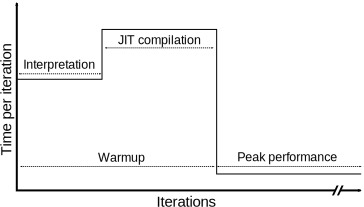
\includegraphics[width=.5\textwidth]{img/picturebook_warmup}
\caption{The traditional notion of warmup: a program starts slowly executing in
an interpreter; once hot parts of the program are identified, they are
translated by the JIT compiler to machine code; at this point warmup
is said to have completed, and peak performance reached.}
\label{fig:trad}
\end{figure}

While some benchmarks on some VMs run as per
traditional expectations, we found a number of surprising cases. At
the most extreme, some benchmarks never warm up, staying at their initial performance
levels indefinitely and some even slowdown. Of the eight
VMs we looked at, none consistently warmed under the traditional model.

Our results clearly invalidate H1: the traditional view of warmup is no longer
valid. We are not aware that anyone has systematically noted this
problem before, let alone take it into account when benchmarking. This suggests
that many published VM benchmarks (including our own) may have presented
results which are misleading in some situations.

We believe that accurate VM benchmarking is paramount, for both VM authors, and
for many end users. VM authors need to know if optimisations have an effect
distinguishable from noise (and many optimisations have only a small effect).
Similarly, end-users with latency sensitive workloads (e.g. games or other soft
real-time systems) rely upon accurate benchmarking during their evaluation
phase. Our results suggest that current benchmarking methodology is leading
these parties astray.

\section{Background}
\label{sec:warmup}

When a program begins running on a JIT compiled VM, it is typically (slowly)
interpreted; once `hot' (i.e.~frequently executed) loops or methods are
identified, they are compiled into machine code; and subsequent
executions of those loops or methods use (fast) machine code rather than the
(slow) interpreter. Once machine code generation has completed, the VM is
traditionally said to have finished warming up, and the program to be executing
at peak performance.\footnote{This traditional notion applies equally to VMs
that perform immediate compilation instead of using an interpreter, and to
those VMs which have more than one layer of JIT compilation (later JIT
compilation is used for `very hot' portions of a program, and tolerates slower
compilation time for better machine code generation).}

Figure~\ref{fig:trad} illustrates a
program subject to the conventional model of warmup. Exactly how long warmup
takes is highly dependent on
the program and the JIT compiler, but this basic assumption about the
performance model is shared by every JIT compiling
VM~\cite{kalibera13rigorous}.

Benchmarking of JIT compiled VMs typically focusses on peak
performance. in large part because the widespread assumption has been that
warmup is both fast and inconsequential to users. With that assumption in mind, the
methodologies used are typically straightforward: benchmarks are run for a number
of in-process iterations within a single VM process execution.
The first $n$ in-process iterations are then discarded, on the basis that warmup
will have completed at some point before $n$. It is common for
$n$ to be a hard-coded number, e.g. 5. The more sophisticated \kalibera
benchmarking methodology~\cite{kalibera12quantifying,kalibera13rigorous}
(recently used in~\cite{barrett15approaches,grimmer15dynamically}) improves
upon this by having the user manually inspect run-sequence plots (or trace
plots) for each process execution. The method also suggests a method for
dealing with benchmarks which are cyclic in nature (e.g. that produce a
saw-tooth wave when plotted).

While the \kalibera methodology is certainly an improvement over
straightforward benchmarking methodologies,
our experience has been that there remain cases where it is hard to produce
satisfying benchmarking statistics. Crucially, the methodology does not
provide a firm way of determining when warmup has completed. Because of this
``determining when a system has warmed up, or even providing a
rigorous definition of the term, is an open research problem''~\cite{seaton15phd}.

\section{Methodology}
\label{sec:methodology}

To test Hypothesis H1, we designed an experiment which uses a suite of
micro-benchmarks: each is run with 2000 in-process iterations and repeated
using 10 process executions. So as
to collect high-quality data, we have carefully designed our
experiment to be repeatable and to control as many potentially confounding variables as
is practical.

In this section we detail: the benchmarks we used and the modifications we
applied; the machines we used for benchmarking; the VMs we benchmarked; and the
\krun system we developed to run benchmarks.


\subsection{The Micro-benchmarks}

The micro-benchmarks we use are as follows: \binarytrees, \spectralnorm, \nbody,
\fasta, and \fannkuch from the Computer Language Benchmarks Game (CLBG); and
\richards. Readers can be forgiven for initial scepticism about this set of micro-benchmarks.
They are small and widely
used by VM authors as optimisation targets. In general they are more effectively
optimised by VMs than average programs; when used as a proxy for other types
of programs (e.g.~large programs), they tend to overstate the effectiveness of
VM optimisations. In our context, this weakness is in fact a strength: we need
small, deterministic, and widely examined programs so that we can test
Hypothesis \hypone. Put another way, if we were to run arbitrary programs
and find unusual warmup behaviour, a VM author might reasonably counter that
``you have found the one program that exhibits unusual warmup behaviour''.

For each benchmark, we provide C, Java, Javascript, Python, Lua, PHP,
and Ruby versions.\footnote{Our need to have implementations in a wide variety
of languages restricted the micro-benchmarks we could use.} Since most of these
benchmarks have multiple implementations in any given language, we picked
the same versions used in~\cite{bolz14impact}, which represented the fastest
performers at the point of that publication. We were forced to skip some
benchmark and VM pairings which either ran prohibitively slowly
(Fasta/JRubyTruffle and Richards/HHVM), or caused the VM to crash
(SpectralNorm/JRubyTruffle).\footnote{Later versions of this paper
will use newer VM versions, which we hope may fix these problems.}
For the avoidance of doubt we
did not interfere with any VM's Garbage Collection (GC) (e.g.~we did not
force a collection after each iteration).


\subsubsection{Ensuring Determinism}

We wish to ensure, as far as possible, that the micro-benchmarks are
deterministic from the user's perspective, by which we mean that they
take precisely the same path through the Control Flow Graph (CFG) on each
execution and iteration. Note that this definition deliberately focuses
on non-determinism that is controllable by the user; other forms of
non-determinism within the VM are deliberately excluded, as they are
part of what we are trying to measure (e.g.~objects in memory may be allocated
or garbage collected non-deterministically). To test this, we created
versions of all benchmarks with \texttt{print} statements at all possible points of
divergence (e.g.~\texttt{if} statements' true and false branches).
These versions are available in our experimental suite.

We first ran the benchmarks with 2 process executions and 20 in-process iterations,
and compared the outputs of the two processes. This was enough to show that the
\fasta benchmark was non-deterministic
in all language variants. This is because \fasta generates random numbers with
a seed that is initialised only at the very start of the benchmark, thus
causing each in-process iteration to generate different random numbers. We
fixed this by moving the random seed initialisation to the start
of the in-process iteration main loop.

Bearing in mind surprising
results such as the importance of link order~\cite{mytkowicz09surprising}, we
then used two different machines to compile VMs and then ran the benchmarks
on these machines.
Using this technique we noticed occasional non-determinism in Java benchmarks.
This ultimately turned out to be caused by lazy class loading. To integrate
the Java benchmarks with \krun (see Section~\ref{krun}), each
benchmark was given an additional \texttt{KrunEntry} class,
which, in essence, provides an interface between \krun and the main benchmark
class. Because of this, the main benchmark class was lazily loaded after
benchmark timing had started (sometimes in a way that we could observe). We
solved this by adding to each benchmark an empty static method, which each
\texttt{KrunEntry} then calls via a static initialiser. In so doing, we
guarantee that the main benchmark class is not lazily loaded. Note that Java
benchmarks -- as well as
Java-based systems such as Graal and JRuby/Truffle -- will still be subject to
lazy loading, which is an inherent part of the JVM specification: forcing all
classes to be eagerly loaded is impractical, and is thus part of the warmup we
wish to measure.

\subsection{Measuring Computation and Not File Performance}

Micro-benchmarks often perform computations which are partly or wholly
irrelevant, i.e. the results of computations are not externally visible. Highly
optimising compilers are thus often able to optimise away part or all of a
micro-benchmark's computation. From a performance standpoint, this is a
desirable characteristic for
optimising compilers~\cite{seaton15phd}, though benchmarks whose computations
are entirely removed are rarely useful. To ensure that computation cannot
be optimised away, many benchmarks write intermediate and final results
to \texttt{stdout}. However, one can quickly end up in a situation where benchmarks are
unintentionally measuring, in part or whole, the performance of file routines in
the OS libraries and the kernel.

To avoid both of these unfortunate cases,
we modified the benchmarks to calculate a checksum during each in-process iteration.
The checksum is validated at the end of each in-process iteration against an expected
value; if the check fails, the incorrect checksum is written to \texttt{stdout}.
By writing benchmarks in
this style, we make it difficult for optimising compilers to remove the
main bulk of the benchmark. Note that each micro-benchmark has a single checksum value for all
language variants, which also provides some assurance that each language variant is
performing the same work.


\subsection{Benchmarking Hardware}

%We used three machines and two operating systems:
We used two benchmarking machines:

\begin{tabular}{ll}
  \bencherthree & Quad-core i7-4790K 4GHz, 24GB of RAM, running Debian 8. \\
  \bencherfive  & Quad-core i7-4790 3.6GHz, 32GB of RAM, running Debian 8.
%  \item[\benchersix] Identical hardware to \bencherfive, but running OpenBSD 5.8.
\end{tabular}

\noindent These machines allow us to investigate the effects of moderately different
hardware (\bencherthree and \bencherfive run the same operating system with the
same updates installed)
%as well as moderately different operating systems
%(\bencherfive and \benchersix have almost identical hardware, but run different
%Unix
%variants). With regards to hardware and operating systems, we started with the
%following hypothesis:
%\begin{description}
%  \item[\hyptwo] Moderately different hardware and operating systems have little effect on warmup patterns.
%\end{description}
%We deliberately use the word `moderately', since significant changes of hardware
%(e.g.~x86 vs.~ARM) or operating system (e.g.~Linux vs.~Windows) implies that
%significantly different parts of the VMs will be used (e.g.~different machine
%code backends may be of differing levels of maturity).

We disabled turbo boost and hyper-threading in the BIOS. Turbo boost is a
feature which allows CPUs to temporarily run in an extremely high-performance
mode; this eventually causes the CPU to exceed its safe thermal limit,
at which point it reduces performance until it has cooled down sufficiently.
Turbo boost can thus cause long-running processes to
appear to suddenly slow down. Hyper-threading gives the illusion that a single
physical core is in fact more than one logical core, inter-leaving the
execution of two or more programs or threads on a single physical core.
Hyper-threading causes programs to interfere
with each others in complex ways, introducing considerable noise.


\subsection{VMs under investigation}

We ran the benchmarks on the following language implementations:

\begin{tabular}{ll}
GCC & Version 4.9.2 (from Debian packages). \\
Graal \#9dafd1dc5ff9 & HotSpot using a next-gen compiler. \\
HHVM 3.7.1 & A JIT compiled VM for PHP. \\
JRuby/Truffle \#7f4cd59cdd1c8 & A Ruby interpreter using Graal for compilation. \\
HotSpot 8u45b14 & The most widely used Java VM. \\
LuaJIT 2.0.4 & A tracing JIT compiler for Lua. \\
PyPy 4.0.0 & A meta-tracing VM for Python 2.7. \\
V8 4.8.271.9 & A JIT compiler for Javascript.
\end{tabular}
\edd[final]{Add to list: CPython 2.7.10, The reference Python implementation}%

\noindent Although not a VM, GCC serves as a baseline to compare the VMs against.

We created a build script which downloads, configures, and builds fixed
versions of the
VMs, ensuring we can easily repeat builds.
All VMs were compiled with GCC/G++ 4.9.2.\edd[final]{Say something about a
fixed GCC across platforms}\edd[final]{Neither HHVM nor
JRuby/Truffle has currently been ported to OpenBSD, and thus we were unable to
run those VMs on OpenBSD.}


\subsection{\krun}
\label{krun}

We developed a tool called \krun to fully automate the running of benchmarks
and to control the environment under which the benchmarks run. \krun itself is a
`supervisor' process which first configures a system before running VM-specific
benchmarks, monitoring the system for any signs of errors during benchmarking,
and writing results to a compressed JSON file. \krun is invoked with a
configuration file which describes the VMs, benchmarks, and number of process
executions and in-process iterations to
be executed.

In the remainder of this subsection, we describe: the variables which \krun
controls (both generic and platform dependent); and how \krun collects data.
Note that, although \krun has `developer' modes which disable various checks,
we describe only the `production' mode, which has all checks enabled.


\subsubsection{Platform Independent Controls}

Several of \krun's controls work on all supported platforms. \krun imposes a
consistent heap and stack \texttt{ulimit} for all
VMs (we used a 2GiB heap and a 8MiB stack).\footnote{Note that Linux allows users
to inspect these values, but to allocate memory beyond them.} Benchmarks are run
as the Unix user `\texttt{krun}', which performs no environment configuration.
\krun reboots the system before each process execution (including
before the first) to ensure that the system is in a somewhat known state
(e.g.~if a benchmark caused a system to transfer memory from RAM to disk-based swap,
rebooting ensures that later benchmarks are not affected). After each reboot, \krun
is invoked automatically by the system's init subsystem; it pauses for 3 minutes to allow the system
to fully initialise before running the next process execution.

\krun performs two types of monitoring before and during benchmark execution.
First, \krun monitors the system's \texttt{dmesg} buffer, informing the user of
any changes. We implemented this feature after noticing that one of the
machines we had earlier ear-marked for running benchmarks occasionally
overheated, with the only clue to this being a message left in the \texttt{dmesg}.
We did not use this machine for our final benchmarking.
Second, \krun monitors temperature sensors. Since modern systems may limit
performance when they get too hot, \krun ensures that all process executions
start at approximately the same temperature. Before the first process execution,
\krun waits for a fixed period of time (60s) in the hope that the machine
cools down; after this point, it collects temperature
readings from all available temperature sensors, which are then used as
base temperature readings. Before each subsequent process execution, \krun
waits until each temperature sensor is within 10\%{} of its base temperature
before continuing. If any sensor fails to meet this threshold
within 10 minutes, \krun terminates the entire experiment.


\subsubsection{Linux-specific Controls}

On Linux, \krun controls several additional factors.

\krun sets the CPU frequency to the highest non-over-clocked value possible.
The user must first disable Intel P-state support in
the kernel by passing the kernel argument \texttt{intel\_pstate=disable}.
\krun verifies P-states are disabled and uses \texttt{cpufreq-set} to set
the CPU governor to \texttt{performance} mode. Note that even with these
options set, we cannot fully guarantee that the CPU does as requested
(see Section~\ref{sec:threats} for details).

\krun checks that it is running on a `tickless' kernel, which aims to reduce
jitter in time-sensitive workloads~\cite{tickless}. The default
Linux kernel interrupts each active logical CPU\footnote{Note that each core of
each individual processor chip counts as a logical CPU.} 250 times (`ticks') a second to
decide whether to perform a context switch. We used a kernel with the
\texttt{CONFIG\_NO\_HZ\_FULL\_ALL} compile-time option set, which puts
all CPUs except one (the boot CPU) into adaptive-tick mode.
CPUs in adaptive-tick mode are only interrupted by the kernel if more than
one runnable process is scheduled.
When we compared a subset of benchmarks on a tickless vs.~a standard
kernel, we noticed a small reduction in jitter, although not enough for us to
conclusively say that the tickless kernel was the cause. However,
since, at worst, it appears to have no negative effects, we ran our experiments
using the tickless kernel.

Linux's \texttt{perf} system dynamically profiles system performance by
repeatedly sampling hardware counters. We became aware of \texttt{perf} when
\krun's \texttt{dmesg} checks notified us that the kernel had decreased the
sample-rate as it determined that it was sampling too often. Since \texttt{perf}
can interrupt benchmarking, its existence is undesirable, particularly since its
effects can vary over time. Although \texttt{perf} cannot be disabled entirely,
\krun sets the sample-rate to the smallest possible value of 1 sample per
second.

Finally, \krun disables Address Space Layout Randomisation (ASLR). While this is
a sensible security precaution for everyday use, it makes it difficult to
compare the performance of even a single binary.\footnote{The Stabilizer
system~\cite{curtsinger13stabilizer} is an intriguing approach for obtaining reliable
statistics in the face of features such as ASLR. Unfortunately we were not able
to build it on a modern Linux system.} \krun sets the
\texttt{randomize\_va\_space} entry in \texttt{/proc} to 0, disabling ASLR
globally.


%\subsubsection{OpenBSD-specific Controls}
%
%Relative to Linux, OpenBSD exposes many fewer knobs to users. Nevertheless,
%there are two OpenBSD specific features in \krun.
%
%First, \krun sets CPU performance to maximum by invoking \texttt{apm -H} prior
%to running benchmarks. This is equivalent to setting Linux's CPU governor to
%\texttt{performance} mode, but note that OpenBSD offers no means of changing
%Intel P-states.
%
%Second, \krun sets OpenBSD's default \texttt{malloc} implementation to be
%deterministic. By default, OpenBSD's \texttt{malloc} performs several operations
%for security purposes, including allocating guard pages and randomising layout.
%We set the \texttt{MALLOC\_OPTIONS} environment variable to \texttt{sfghjpru},
%turning it into a more traditional, and hopefully largely deterministic,
%\texttt{malloc}.


\subsubsection{The Iterations Runners}

Since we run benchmarks in several different languages, we need a way to report
timings from benchmarks to \krun. For each language, we created an
\emph{in-process iterations runner}. When \krun wants to run a benchmark, it executes the
appropriate in-process iterations runner for that language, passing it the name of the
benchmark to be run, and the desired number of in-process iterations. The in-process iterations runner
then dynamically loads the benchmark, and repeatedly executes the main body of
the benchmark. The in-process iterations runner calls a monotonic timer with
sub-millisecond accuracy before and after each in-process iteration, printing timing
data to \texttt{stdout}; when all iterations are complete, \krun consumes
the timing data and stores it into a compressed JSON file.

Most VMs expose the low-level monotonic timing function \texttt{clock\_gettime}
(which our iterations runners use) to the target language as standard. We
extended V8, HHVM and JRuby/Truffle
to expose this monotonic clock via a user-visible function.
On OpenBSD, we use the \texttt{CLOCK\_MONOTONIC} timer; on Linux this timer is subject to
interference from the \texttt{adjtime} function, and we thus use the
\texttt{CLOCK\_MONOTONIC\_RAW} timer.

\begin{figure}[t]
\begin{lstlisting}
iter_times = [-1.0] * iters
for i in xrange(iters):
  start_time = clock_gettime_monotonic()
  call_iteration()
  stop_time = clock_gettime_monotonic()
  iter_times[i] = stop_time - start_time

sys.stdout.write("[%s]" % ",".join([str(x) for x in iter_times]))
\end{lstlisting}
\caption{An elided example of the in-process iteration runner for Python. As
this shows, the core loop is extremely minimal to minimise the introduction of
timing noise and distortion. Note that the \texttt{iter\_times} array is
pre-allocated to a fixed size, so no array reallocation happens in the core
loop; and that the timing data is only written once all in-process iterations
are complete.}
\label{fig:pythonitsrunner}
\end{figure}

A deliberate design goal of the in-process iterations runners is to minimise the
introduction of timing noise and distortion. First, we do not make any system
calls other than to \texttt{clock\_gettime}. System calls require the CPU to
switch from user mode to kernel mode, and then execute an arbitrary amount
of code; on Linux, calling complex functions as \texttt{write} can evict as much
as two thirds of an x86's vital L1 cache~\cite{soares10flexsc}, as well as
increasing the chances of a full process context switch (which is significantly
slower than a mere mode switch). Second, we allocate the minimum possible memory in
the core loop (in some languages, we allocate no memory; in others, we are
unable to remove the memory needed for basic items such as integers). In
conjunction, these two design goals mean that we pre-allocate an array of floats
with one entry per in-process iteration before the core loop. After each
in-process iteration, the relevant entry is updated in the array. After
all in-process iterations have completed, the total array is printed to
\texttt{stdout}. Figure~\ref{fig:pythonitsrunner} shows an elided version
of the Python in-process iterations runner, embodying these design goals.



\bibliographystyle{plainnat}
\bibliography{bib}

\end{document}

